\documentclass[11pt,a4paper]{article}

\usepackage[utf8]{inputenc}
\usepackage[T1]{fontenc}
\usepackage{lmodern}
\usepackage{amsmath,amssymb,amsfonts}
\usepackage{booktabs}
\usepackage{multirow}
\usepackage{graphicx}
\usepackage{xcolor}
\usepackage{tikz}
\usetikzlibrary{arrows.meta,positioning,calc,fit,backgrounds,shapes.geometric,decorations.pathreplacing}
\usepackage[margin=1in]{geometry}
\usepackage{hyperref}
\usepackage{enumitem}
\usepackage{microtype}
\usepackage{caption}
\usepackage{subcaption}
\usepackage[numbers,sort&compress]{natbib}
\usepackage{url}

\hypersetup{colorlinks=true,linkcolor=blue!60!black,citecolor=blue!60!black,urlcolor=blue!60!black}

\definecolor{nvgreen}{RGB}{118,185,0}
\definecolor{codebookblue}{RGB}{41,128,185}

\title{\textbf{CBINT2: Sub-3-Bit Weight Compression\\for NVFP4 Tensor Cores}\\[6pt]
\large Research Proposal --- Draft for Discussion}

\author{Huanchen Sun \and Junzhou He}
\date{}

\begin{document}
\maketitle

% ===========================================================================
\begin{abstract}
\begin{sloppypar}
NVFP4 tensor cores on Blackwell GPUs deliver $2\text{--}3\times$ the throughput of BF16, but at 4.5 bits per element, NVFP4 weights remain the memory-bandwidth bottleneck---especially for MoE models where per-expert batch sizes are small.
We propose \textbf{CBINT2}: quantize from \textbf{BF16 or NVFP4} down to \textbf{3.0 bits/element}, then \emph{dequantize back to NVFP4 at runtime with near-zero overhead} via a register-resident table lookup feeding FP4 tensor cores directly.
Prior sub-4-bit methods (QuIP\#, AQLM, QTIP) dequantize to BF16 with large codebooks and expensive kernels, then run on slower tensor cores.
CBINT2 stores at 3 bits, computes at FP4 speed.
Preliminary results on Qwen3-30B-A3B show $-$0.87pt on GSM8K with naive codebook selection; GPTQ calibration and direct BF16 quantization are expected to close the remaining gap.
We target \textbf{ASPLOS 2026}.
\end{sloppypar}
\end{abstract}

% ===========================================================================
\section{Introduction}
\label{sec:intro}

LLM inference is memory-bandwidth bound: each decoded token loads the full weight matrix~\cite{dettmers2023kbit}.
NVFP4 (FP4-E2M1) tensor cores on Blackwell~\cite{nvidia2025nvfp4} deliver $2\text{--}3\times$ higher throughput than BF16 at near-lossless accuracy~\cite{nvidia2026nvfp4accelerates}, making NVFP4 the \emph{de facto} inference standard at 4.5 bits/element.
Yet weight loading remains the bottleneck for MoE models, where sparse activation produces small per-expert batches.

Prior 2-bit methods (QuIP\#~\cite{tseng2024quipsharp}, AQLM~\cite{egiazarian2024aqlm}, QTIP~\cite{tseng2024qtip}, GPTVQ~\cite{vanbaalen2024gptvq}) all \textbf{dequantize to BF16/FP16}---requiring large codebook lookups ($2^{8}$--$2^{16}$ entries), floating-point reconstruction on CUDA cores (20--90\% overhead~\cite{lin2025qserve}), and execution on slower BF16 tensor cores.

\textbf{Our key observation:} NVFP4 has only \textbf{16 representable values}.
This makes it uniquely suited as a \emph{runtime decompression target}: the entire alphabet fits in registers, lookup is a trivial integer operation, and the output feeds FP4 tensor cores directly.
The core idea: \textbf{quantize from BF16 or NVFP4 $\to$ store at $\sim$3 bits $\to$ dequantize to NVFP4 at runtime with near-zero overhead $\to$ FP4 tensor core compute.}
No prior sub-4-bit method targets NVFP4 as the decompression format.

% ===========================================================================
\section{Codebook Design}
\label{sec:method}

\textbf{NVFP4 format.}
Each block of 16 FP4-E2M1 elements (magnitudes $\{0, 0.5, 1, 1.5, 2, 3, 4, 6\}$ $\times$ sign = 15 values) is stored with an FP8-E4M3 per-group scale and an FP32 per-tensor global scale.
Dequantization: $W = \text{fp4} \times (\text{scale} / \text{global\_scale})$.
Cost: $(16 \times 4 + 8)/16 = 4.5$ bits/element.

\textbf{Core idea.}
Restrict each 16-element block from 15 values to \textbf{4} (zero $+$ 3 chosen non-zero values) $\to$ 2 bits per element.
Selecting 3 from 14 non-zero values gives $\binom{14}{3} = 364$ candidates; sign symmetry (negate scale) folds this to \textbf{182 codebooks}, encoded in 8 bits.
For each block, we try all 182 candidates and pick the one minimizing MSE.

\textbf{Two quantization paths.}
(i)~\emph{NVFP4$\to$CBINT2}: compress existing NVFP4 checkpoints (inherited scale).
(ii)~\emph{BF16$\to$CBINT2} (proposed): jointly optimize scale, codebook, and element mapping against full-precision weights---strictly stronger.

\begin{figure}[t]
\centering
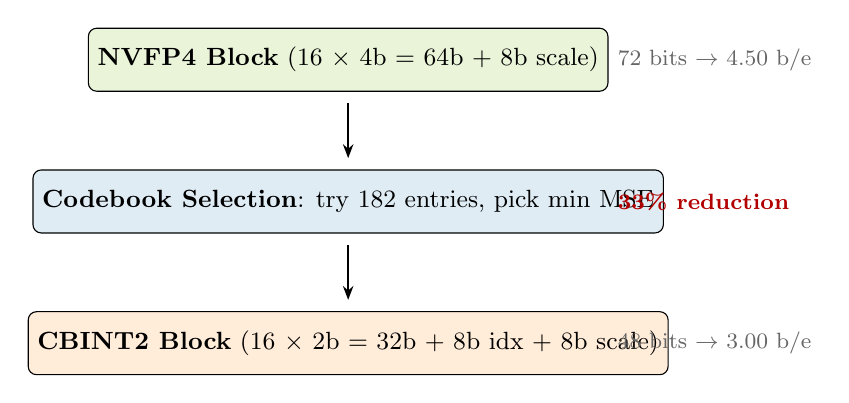
\begin{tikzpicture}[
    box/.style={draw, rounded corners=3pt, minimum height=0.8cm, text centered, font=\small},
    arr/.style={-{Stealth[length=5pt]}, thick},
    every node/.style={font=\small}
]
\node[box, fill=nvgreen!15, minimum width=5.5cm] (orig) at (0,0) {
    \textbf{NVFP4 Block} (16 $\times$ 4b = 64b + 8b scale)
};
\draw[arr] (0,-0.55) -- (0,-1.25);
\node[box, fill=codebookblue!15, minimum width=5.5cm] (select) at (0,-1.8) {
    \textbf{Codebook Selection}: try 182 entries, pick min MSE
};
\draw[arr] (0,-2.35) -- (0,-3.05);
\node[box, fill=orange!15, minimum width=5.5cm] (cb) at (0,-3.6) {
    \textbf{CBINT2 Block} (16 $\times$ 2b = 32b + 8b idx + 8b scale)
};
\node[font=\footnotesize, anchor=west, text=black!60] at (3.3, 0) {72 bits $\to$ 4.50 b/e};
\node[font=\footnotesize, anchor=west, text=black!60] at (3.3, -3.6) {48 bits $\to$ 3.00 b/e};
\node[font=\footnotesize\bfseries, anchor=west, text=red!70!black] at (3.3, -1.8) {33\% reduction};
\end{tikzpicture}
\caption{CBINT2 compresses each 16-element NVFP4 block from 72 to 48 bits.}
\label{fig:pipeline}
\end{figure}

\textbf{Bit budget and sharing.}
Table~\ref{tab:bitbudget} shows the per-block cost.
The 8-bit codebook index can be amortized across $K$ adjacent blocks via lossy sharing (Table~\ref{tab:sharing}), tracing a rate--distortion curve from 3.0 bits ($K$=1) to 2.5 bits ($K\to\infty$).

\begin{table}[t]
\centering
\begin{minipage}[t]{0.48\textwidth}
\centering
\caption{Per-block bit budget.}
\label{tab:bitbudget}
\begin{tabular}{lcc}
\toprule
 & \textbf{NVFP4} & \textbf{CBINT2} \\
\midrule
Values & 64 & 32 \\
Codebook idx & --- & 8 \\
Scale (FP8) & 8 & 8 \\
\midrule
\textbf{Total} & \textbf{72} & \textbf{48} \\
\textbf{Bits/elem} & \textbf{4.50} & \textbf{3.00} \\
\bottomrule
\end{tabular}
\end{minipage}\hfill
\begin{minipage}[t]{0.48\textwidth}
\centering
\caption{Codebook sharing ($K$ blocks).}
\label{tab:sharing}
\begin{tabular}{ccc}
\toprule
$K$ & \textbf{Bits/e} & \textbf{Speedup} \\
\midrule
1 & 3.00 & $1.50\times$ \\
2 & 2.75 & $1.64\times$ \\
4 & 2.625 & $1.71\times$ \\
8 & 2.5625 & $1.76\times$ \\
\bottomrule
\end{tabular}
\end{minipage}
\end{table}

% ===========================================================================
\section{Fused Decompression}
\label{sec:kernel}

\begin{figure}[t]
\centering
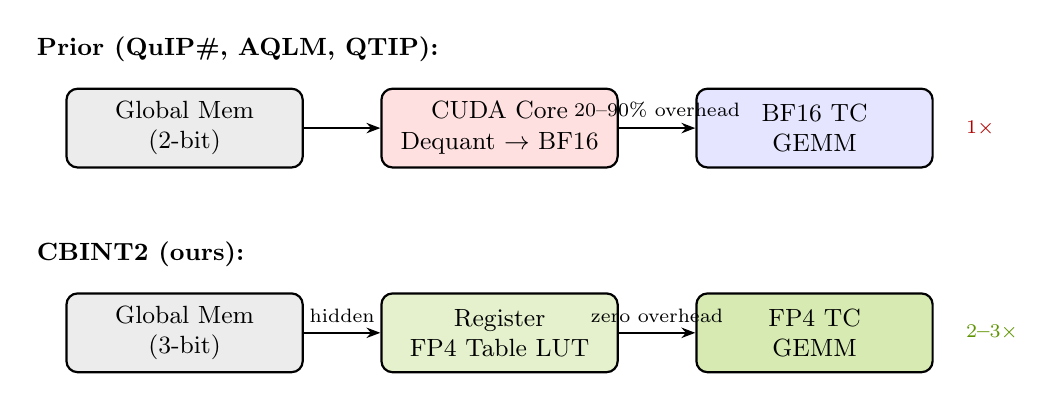
\begin{tikzpicture}[
    stage/.style={draw, rounded corners=4pt, minimum height=1.0cm, minimum width=3.0cm, align=center, font=\small, thick},
    arr/.style={-{Stealth[length=5pt]}, thick},
]
\node[font=\small\bfseries, anchor=west] at (-5.3, 2.3) {Prior (QuIP\#, AQLM, QTIP):};
\node[stage, fill=gray!15] (mem1) at (-3.3, 1.3) {Global Mem\\(2-bit)};
\node[stage, fill=red!12] (dq1) at (0.7, 1.3) {CUDA Core\\Dequant $\to$ BF16};
\node[stage, fill=blue!10] (tc1) at (4.7, 1.3) {BF16 TC\\GEMM};
\draw[arr] (mem1) -- (dq1);
\draw[arr] (dq1) -- (tc1) node[midway, above, font=\scriptsize] {20--90\% overhead};

\node[font=\small\bfseries, anchor=west] at (-5.3, -0.3) {CBINT2 (ours):};
\node[stage, fill=gray!15] (mem2) at (-3.3, -1.3) {Global Mem\\(3-bit)};
\node[stage, fill=nvgreen!20] (dq2) at (0.7, -1.3) {Register\\FP4 Table LUT};
\node[stage, fill=nvgreen!30] (tc2) at (4.7, -1.3) {FP4 TC\\GEMM};
\draw[arr] (mem2) -- (dq2) node[midway, above, font=\scriptsize] {hidden};
\draw[arr] (dq2) -- (tc2) node[midway, above, font=\scriptsize] {zero overhead};

\node[font=\scriptsize, text=red!70!black, anchor=west] at (6.5, 1.3) {$1\times$};
\node[font=\scriptsize\bfseries, text=nvgreen!80!black, anchor=west] at (6.5, -1.3) {$2\text{--}3\times$};
\end{tikzpicture}
\caption{Prior methods dequant to BF16 on CUDA cores; CBINT2 decodes to FP4 in registers and feeds FP4 tensor cores directly.}
\label{fig:kernel}
\end{figure}

CBINT2 decompression: read the 8-bit codebook index $\to$ look up 3 FP4 values from a 182-entry register-resident table (273 bytes) $\to$ write FP4 nibbles via 2-bit element indices $\to$ feed the FP4 MMA instruction.
All operations are integer/bitwise---no FP units consumed.
In a fused GroupGEMM kernel, this decode overlaps with global memory loads at zero effective latency.

% ===========================================================================
\section{Preliminary Results}
\label{sec:prelim}

Results below use the \textbf{simplest configuration}: NVFP4$\to$CBINT2, naive MSE, no GPTQ, expert weights only---a lower bound on CBINT2 accuracy.

\begin{table}[t]
\centering
\caption{NVIDIA-reported BF16 vs.\ NVFP4 accuracy on Qwen3-30B-A3B (NVFP4 is near-lossless).}
\label{tab:nvidia_accuracy}
\resizebox{\textwidth}{!}{
\begin{tabular}{lccccccc}
\toprule
 & \textbf{MMLU Pro} & \textbf{GPQA-D} & \textbf{HLE} & \textbf{LCB} & \textbf{SciCode} & \textbf{MATH-500} & \textbf{AIME'24} \\
\midrule
BF16 & 78.0 & 62.0 & 7.0 & 51.0 & 28.0 & 96.0 & 75.0 \\
NVFP4 & 77.0 & 61.0 & 5.0 & 65.0 & 32.0 & 96.0 & 80.0 \\
\bottomrule
\end{tabular}
}
\end{table}

\begin{table}[t]
\centering
\begin{minipage}[t]{0.48\textwidth}
\centering
\caption{CBINT2 accuracy (naive MSE).}
\label{tab:cbint2_accuracy}
\begin{tabular}{lccc}
\toprule
 & \textbf{NVFP4} & \textbf{CBINT2} & $\Delta$ \\
\midrule
GSM8K & 86.81 & 85.94 & $-$0.87 \\
MMLU & 78.32 & 74.08 & $-$4.24 \\
\bottomrule
\end{tabular}
\end{minipage}\hfill
\begin{minipage}[t]{0.48\textwidth}
\centering
\caption{Effective throughput comparison.}
\label{tab:speedup}
\begin{tabular}{lcc}
\toprule
\textbf{Method} & \textbf{b/w} & \textbf{Eff.\ speedup} \\
\midrule
NVFP4 & 4.50 & $1.00\times$ \\
MARLIN~\cite{frantar2024marlin} & 4.00 & $0.56\times$ \\
QuIP\#~\cite{tseng2024quipsharp} & 2.00 & $1.13\times$ \\
\midrule
\textbf{CBINT2} & \textbf{3.00} & $\mathbf{1.50\times}$ \\
\bottomrule
\end{tabular}
\end{minipage}
\end{table}

GSM8K drops only 0.87pt ($-$1\%).
MMLU drops 4.24pt, expected to improve substantially with GPTQ calibration and direct BF16 quantization.
Effective throughput (Table~\ref{tab:speedup}) accounts for both bandwidth \emph{and} tensor core speed: CBINT2 at 3.0 bits on FP4 TC outperforms QuIP\#/AQLM at 2.0 bits on BF16 TC.

% --- KEY VISUAL: Effective speedup bar chart ---
\begin{figure}[t]
\centering
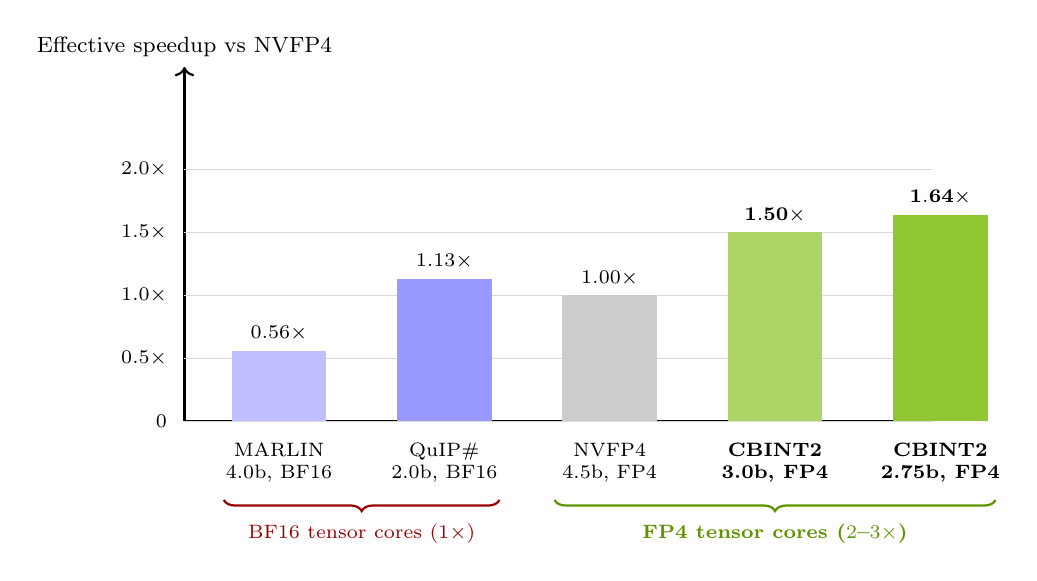
\begin{tikzpicture}[
    every node/.style={font=\small},
]
% Axes
\draw[thick, ->] (0,0) -- (0,4.5) node[above, font=\footnotesize] {Effective speedup vs NVFP4};
\draw[thick] (0,0) -- (9.5,0);

% Gridlines
\foreach \y/\lab in {0/0, 0.8/0.5$\times$, 1.6/1.0$\times$, 2.4/1.5$\times$, 3.2/2.0$\times$} {
    \draw[gray!30] (0,\y) -- (9.5,\y);
    \node[anchor=east, font=\scriptsize] at (-0.1,\y) {\lab};
}

% Bars: width 1.2, gap 0.6
% MARLIN W4A16: 0.56x -> 0.56*1.6=0.896
\fill[blue!25] (0.6,0) rectangle (1.8, 0.896);
\node[font=\scriptsize, anchor=south] at (1.2, 0.896) {$0.56\times$};
\node[font=\scriptsize, anchor=north, align=center] at (1.2, -0.15) {MARLIN\\4.0b, BF16};

% QuIP#/AQLM: 1.13x -> 1.13*1.6=1.808
\fill[blue!40] (2.7,0) rectangle (3.9, 1.808);
\node[font=\scriptsize, anchor=south] at (3.3, 1.808) {$1.13\times$};
\node[font=\scriptsize, anchor=north, align=center] at (3.3, -0.15) {QuIP\#\\2.0b, BF16};

% NVFP4 baseline: 1.0x -> 1.6
\fill[gray!40] (4.8,0) rectangle (6.0, 1.6);
\node[font=\scriptsize, anchor=south] at (5.4, 1.6) {$1.00\times$};
\node[font=\scriptsize, anchor=north, align=center] at (5.4, -0.15) {NVFP4\\4.5b, FP4};

% CBINT2 K=1: 1.50x -> 2.4
\fill[nvgreen!60] (6.9,0) rectangle (8.1, 2.4);
\node[font=\scriptsize\bfseries, anchor=south] at (7.5, 2.4) {$\mathbf{1.50\times}$};
\node[font=\scriptsize\bfseries, anchor=north, align=center] at (7.5, -0.15) {\textbf{CBINT2}\\3.0b, FP4};

% CBINT2 K=2: 1.64x -> 2.624
\fill[nvgreen!80] (9.0,0) rectangle (10.2, 2.624);
\node[font=\scriptsize\bfseries, anchor=south] at (9.6, 2.624) {$\mathbf{1.64\times}$};
\node[font=\scriptsize\bfseries, anchor=north, align=center] at (9.6, -0.15) {\textbf{CBINT2}\\2.75b, FP4};

% Bracket annotation: "BF16 TC" vs "FP4 TC"
\draw[decorate, decoration={brace, amplitude=4pt, mirror}, thick, red!60!black]
    (0.5, -1.0) -- (4.0, -1.0) node[midway, below=5pt, font=\scriptsize, text=red!60!black] {BF16 tensor cores ($1\times$)};
\draw[decorate, decoration={brace, amplitude=4pt, mirror}, thick, nvgreen!80!black]
    (4.7, -1.0) -- (10.3, -1.0) node[midway, below=5pt, font=\scriptsize\bfseries, text=nvgreen!80!black] {FP4 tensor cores ($2\text{--}3\times$)};
\end{tikzpicture}
\caption{\textbf{The key result:} effective throughput accounts for both compression ratio \emph{and} tensor core speed. CBINT2 at 3.0 bits on FP4 TC outperforms QuIP\#/AQLM at 2.0 bits on BF16 TC by $1.33\times$. Prior methods are on the wrong compute path.}
\label{fig:speedup}
\end{figure}

% --- VISUAL: Accuracy bar chart ---
\begin{figure}[t]
\centering
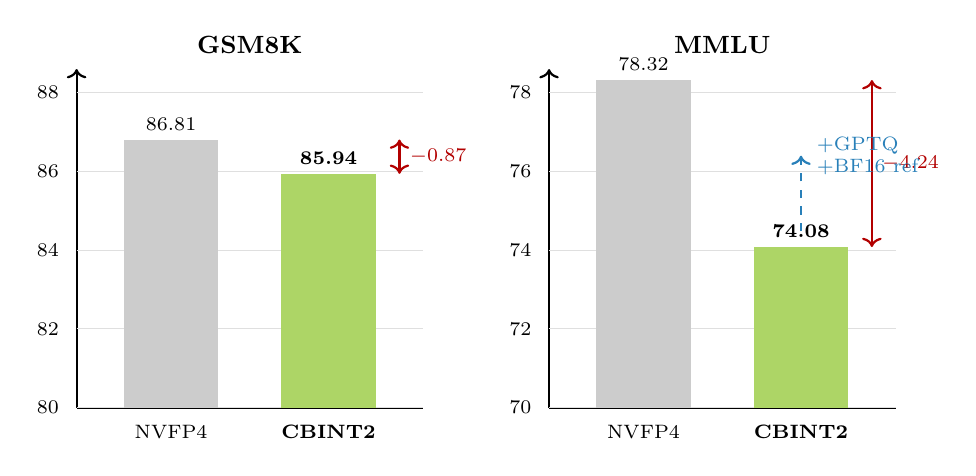
\begin{tikzpicture}[every node/.style={font=\small}]
% --- GSM8K subplot (left) ---
\node[font=\small\bfseries] at (2.2, 4.6) {GSM8K};
\draw[thick,->] (0,0) -- (0,4.3);
\draw[thick] (0,0) -- (4.4,0);
% Y axis: 80 to 90
\foreach \y/\lab in {0/80, 1/82, 2/84, 3/86, 4/88} {
    \draw[gray!25] (0,\y) -- (4.4,\y);
    \node[anchor=east, font=\scriptsize] at (-0.1,\y) {\lab};
}
% NVFP4: 86.81 -> (86.81-80)/2 = 3.405
\fill[gray!40] (0.6,0) rectangle (1.8, 3.405);
\node[font=\scriptsize] at (1.2, 3.605) {86.81};
\node[font=\scriptsize, anchor=north] at (1.2, -0.1) {NVFP4};
% CBINT2: 85.94 -> (85.94-80)/2 = 2.97
\fill[nvgreen!60] (2.6,0) rectangle (3.8, 2.97);
\node[font=\scriptsize\bfseries] at (3.2, 3.17) {85.94};
\node[font=\scriptsize\bfseries, anchor=north] at (3.2, -0.1) {CBINT2};
% Delta
\draw[<->, thick, red!70!black] (4.1, 2.97) -- (4.1, 3.405)
    node[midway, right, font=\scriptsize, text=red!70!black] {$-$0.87};

% --- MMLU subplot (right) ---
\begin{scope}[xshift=6cm]
\node[font=\small\bfseries] at (2.2, 4.6) {MMLU};
\draw[thick,->] (0,0) -- (0,4.3);
\draw[thick] (0,0) -- (4.4,0);
% Y axis: 70 to 80
\foreach \y/\lab in {0/70, 1/72, 2/74, 3/76, 4/78} {
    \draw[gray!25] (0,\y) -- (4.4,\y);
    \node[anchor=east, font=\scriptsize] at (-0.1,\y) {\lab};
}
% NVFP4: 78.32 -> (78.32-70)/2 = 4.16
\fill[gray!40] (0.6,0) rectangle (1.8, 4.16);
\node[font=\scriptsize] at (1.2, 4.36) {78.32};
\node[font=\scriptsize, anchor=north] at (1.2, -0.1) {NVFP4};
% CBINT2: 74.08 -> (74.08-70)/2 = 2.04
\fill[nvgreen!60] (2.6,0) rectangle (3.8, 2.04);
\node[font=\scriptsize\bfseries] at (3.2, 2.24) {74.08};
\node[font=\scriptsize\bfseries, anchor=north] at (3.2, -0.1) {CBINT2};
% Delta
\draw[<->, thick, red!70!black] (4.1, 2.04) -- (4.1, 4.16)
    node[midway, right, font=\scriptsize, text=red!70!black] {$-$4.24};
% "Expected to improve" annotation
\draw[->, thick, dashed, codebookblue] (3.2, 2.24) -- (3.2, 3.2)
    node[right, font=\scriptsize, text=codebookblue, align=left, xshift=2pt] {+GPTQ\\+BF16 ref};
\end{scope}
\end{tikzpicture}
\caption{Preliminary accuracy (naive MSE, no calibration). GSM8K drops only 0.87pt. MMLU gap (4.24pt) is expected to close with GPTQ calibration and direct BF16$\to$CBINT2 quantization (dashed arrow).}
\label{fig:accuracy}
\end{figure}

% ===========================================================================
\section{Proposed Research Agenda}
\label{sec:agenda}

\textbf{(1) GPTQ-calibrated codebook selection} (\S\ref{sec:agenda}\,.\,1).
\label{sec:agenda:gptq}
Replace naive MSE with Hessian-weighted selection~\cite{frantar2023gptq} in two modes: \emph{NVFP4-reference} (minimize deviation from FP4 baseline) and \emph{BF16-reference} (optimize against full-precision target).
An existing FP4-adapted GPTQ implementation provides the core machinery; the modification is replacing the scalar FP4 rounding with our codebook selection.

\textbf{(2) Direct BF16$\to$CBINT2 quantization.}
\label{sec:agenda:bf16}
\begin{sloppypar}
Quantize directly from BF16, jointly optimizing three degrees of freedom: (i)~the FP8 per-block scale (tuned for 4-value codebook, not 16-value FP4 grid), (ii)~codebook assignment, and (iii)~2-bit element mapping.
This eliminates cascaded error from BF16$\to$NVFP4$\to$CBINT2 and positions CBINT2 as a first-class quantization scheme comparable to QuIP\#/AQLM but targeting FP4 tensor cores.
The NVFP4$\to$CBINT2 path remains valuable for NVFP4-native models.
\end{sloppypar}

\textbf{(3) Codebook sharing sweep.}
\label{sec:agenda:sharing}
Characterize the rate--distortion curve over $K \in \{1,2,4,8,16\}$ with GPTQ calibration, providing a deployment-time rate knob.

\textbf{(4) Whole-model compression.}
\label{sec:agenda:wholmodel}
Extend beyond MoE expert weights to: (i)~\emph{KV cache}---compress from 4.5 to 3.0 bits for $1.5\times$ longer context or more concurrent requests, requiring TRT-LLM attention kernel changes; (ii)~\emph{QKV/O projections}---dense layers accessed every token, independently tunable sharing $K$.

\textbf{(5) Fused GroupGEMM kernel.}
\label{sec:agenda:kernel}
CUTLASS-based kernel fusing codebook decode into the SMEM fill stage on Blackwell, hiding decode in the memory-load pipeline.

% ===========================================================================
\section{Related Work}

\textbf{4-bit quantization.}
GPTQ~\cite{frantar2023gptq}, AWQ~\cite{lin2024awq}, SqueezeLLM~\cite{kim2024squeezellm} target INT4/FP4 but do not compress below 4 bits.

\textbf{Sub-4-bit VQ.}
QuIP\#~\cite{tseng2024quipsharp}, AQLM~\cite{egiazarian2024aqlm}, QTIP~\cite{tseng2024qtip}, GPTVQ~\cite{vanbaalen2024gptvq} all dequantize to BF16/FP16---limiting throughput on FP4 hardware.

\textbf{NVFP4.}
Four Over Six~\cite{cook2025fouroversix} and RaZeR~\cite{chen2026razer} improve NVFP4 accuracy but do not compress below 4.5 bits.

\textbf{Kernels.}
QServe~\cite{lin2025qserve} quantifies 20--90\% dequant overhead; MARLIN~\cite{frantar2024marlin} optimizes W4A16; CodeGEMM~\cite{park2025codegemm} eliminates VQ dequant via precomputed partial sums.
FP4-native decompression eliminates the need for all of these.

% ===========================================================================
\section{Timeline}

\begin{table}[h]
\centering
\caption{Proposed timeline targeting ASPLOS 2026.}
\label{tab:timeline}
\begin{tabular}{lll}
\toprule
\textbf{Phase} & \textbf{When} & \textbf{Deliverable} \\
\midrule
Arxiv preprint & Now & Core idea + preliminary results \\
GPTQ integration & Apr & Both ref modes, full benchmarks \\
Sharing sweep & Apr--May & Rate--distortion curve ($K$=1..16) \\
Fused kernel & May--Jun & GroupGEMM + latency numbers \\
QKV/O + KV cache & Jun--Jul & TRT-LLM integration \\
BF16$\to$CBINT2 & Jun--Jul & Joint scale-codebook pipeline \\
Paper & Jul--Aug & Full ASPLOS submission \\
\bottomrule
\end{tabular}
\end{table}

% ===========================================================================
\section{Conclusion}

\begin{sloppypar}
CBINT2 quantizes from BF16 or NVFP4 to 3 bits and dequantizes back to NVFP4 at runtime with near-zero overhead---store at 3 bits, compute at FP4 speed.
Preliminary results ($-$0.87pt GSM8K with naive selection) validate the idea.
The proposed agenda---GPTQ calibration, direct BF16 quantization, whole-model compression, and fused kernels---will close the accuracy gap and deliver end-to-end speedups for ASPLOS 2026.
\end{sloppypar}

\begin{thebibliography}{16}
\bibitem[Frantar et~al.(2023)]{frantar2023gptq}
E.~Frantar et~al. {GPTQ}: Accurate post-training quantization for generative pre-trained transformers. \emph{ICLR}, 2023.

\bibitem[Lin et~al.(2024)]{lin2024awq}
J.~Lin et~al. {AWQ}: Activation-aware weight quantization for on-device {LLM} compression. \emph{MLSys}, 2024.

\bibitem[Tseng et~al.(2024a)]{tseng2024quipsharp}
A.~Tseng et~al. {QuIP\#}: Even better {LLM} quantization with {Hadamard} incoherence and lattice codebooks. \emph{ICML}, 2024.

\bibitem[Egiazarian et~al.(2024)]{egiazarian2024aqlm}
V.~Egiazarian et~al. Extreme compression of large language models via additive quantization. \emph{ICML}, 2024.

\bibitem[Tseng et~al.(2024b)]{tseng2024qtip}
A.~Tseng et~al. {QTIP}: Quantization with trellises and incoherence processing. \emph{NeurIPS}, 2024.

\bibitem[van Baalen et~al.(2024)]{vanbaalen2024gptvq}
M.~van Baalen et~al. {GPTVQ}: The blessing of dimensionality for {LLM} quantization. \emph{arXiv:2402.15319}, 2024.

\bibitem[Lin et~al.(2025)]{lin2025qserve}
Y.~Lin et~al. {QServe}: {W4A8KV4} quantization and system co-design for efficient {LLM} serving. \emph{MLSys}, 2025.

\bibitem[Frantar et~al.(2024)]{frantar2024marlin}
E.~Frantar et~al. {MARLIN}: Mixed-precision auto-regressive parallel inference on large language models. \emph{ICML}, 2024.

\bibitem[Cook et~al.(2025)]{cook2025fouroversix}
J.~Cook et~al. Four over six: More accurate {NVFP4} quantization with adaptive block scaling. \emph{arXiv:2512.02010}, 2025.

\bibitem[Park et~al.(2025)]{park2025codegemm}
G.~Park et~al. {CodeGEMM}: A codebook-centric approach to efficient {GEMM} in quantized {LLMs}. \emph{NeurIPS}, 2025.

\bibitem[Chen et~al.(2026)]{chen2026razer}
H.~Chen et~al. {RaZeR}: Pushing the limits of {NVFP4} quantization. \emph{ICML}, 2026.

\bibitem[Dettmers and Zettlemoyer(2023)]{dettmers2023kbit}
T.~Dettmers and L.~Zettlemoyer. The case for 4-bit precision: k-bit inference scaling laws. \emph{ICML}, 2023.

\bibitem[Kim et~al.(2024)]{kim2024squeezellm}
S.~Kim et~al. {SqueezeLLM}: Dense-and-sparse quantization. \emph{ICML}, 2024.

\bibitem[{NVIDIA}(2025)]{nvidia2025nvfp4}
{NVIDIA}. Introducing {NVFP4} for efficient and accurate low-precision inference, 2025.

\bibitem[{NVIDIA}(2026)]{nvidia2026nvfp4accelerates}
{NVIDIA}. 3 ways {NVFP4} accelerates {AI} training and inference, 2026.

\bibitem[{Qwen Team}(2025)]{qwen2025qwen3}
{Qwen Team}. Qwen3 technical report, 2025. \url{https://huggingface.co/Qwen/Qwen3-30B-A3B}.
\end{thebibliography}

\end{document}
